% specify the document type
\documentclass{article}[12pt]
\usepackage[utf8]{inputenc}

% include a set of useful packages
\usepackage{graphicx}
\usepackage{amsmath}
\usepackage{amssymb}
\usepackage{cancel}
\usepackage{algorithm2e}
\usepackage{float}
\usepackage{caption}
\usepackage{fancyvrb}
\usepackage[toc,page]{appendix}
\usepackage{hyperref}
\usepackage{subfig}
\usepackage{color}
\usepackage[export]{adjustbox}
\usepackage{multicol}

% define some useful commands
\newcommand{\bvec}[1]{\boldsymbol{#1}}

% setup paths for images
\graphicspath{ {../images/} }

%
% start the presentation
%

% define the title that will be used in the report
\title{QBX and the DPIE for the Maxwell Equations \\  University of Illinois @ Urbana-Champaign\\ Fall 2017 - CS 598 APK}
\author{
	Christian Howard \\ howard28@illinois.edu
}
\date{} % don't set a date because we don't need this shit

% begin the actual document
\begin{document}
	
	% create the title page 
	\maketitle
	\begin{abstract}
		A set of classifiers were built that could be used to predict if an individual has Major Depression given fMRI data about them performing a set of tasks. To accomplish this task, a dense fMRI dataset was coarsened via a local voxel averaging scheme and then features were discovered using Principal Component Analysis (PCA) and Non-negative Matrix Factorization (NMF). Using the new feature representations, classifiers were constructed using the following approaches: Random Forests (RFs), Gaussian Discriminant Analysis (GDA), and a Deep Neural Network (DNN). All of the above classification methods had high testing accuracy. This high accuracy was interesting and appears to stem from the feature representation causing the reduced data to be very separable with respect to their classes.
	\end{abstract}
	\newpage
	
	% project goal
	
	\section{The Goal}
	For this project, the goals were to implement a model for the Python package \textbf{pytential} for tackling the Maxwell Equations for perfect conductors using QBX and the Decoupled Potential Integral Equation (DPIE) formulation. The main expectation with using this model, versus the Magnetic Field Integral Equation (MFIE), is better resolution and convergence across different frequencies.
	
	

	
	% slides talking about motivation
	
	\section{A Little Context}
	Building cool stuff like radars, missiles antennas, medical imaging tech, and more benefit a lot from solving the Maxwell Equations to solve some tough Computational Electromagnetics problems
	
	\vspace{0.5in}
	\hfil\hfil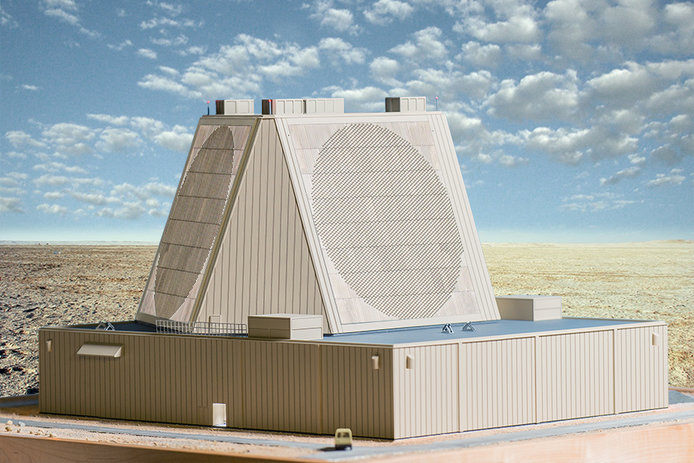
\includegraphics[width=5cm,frame]{raytheonRadar}\hfil\hfil
	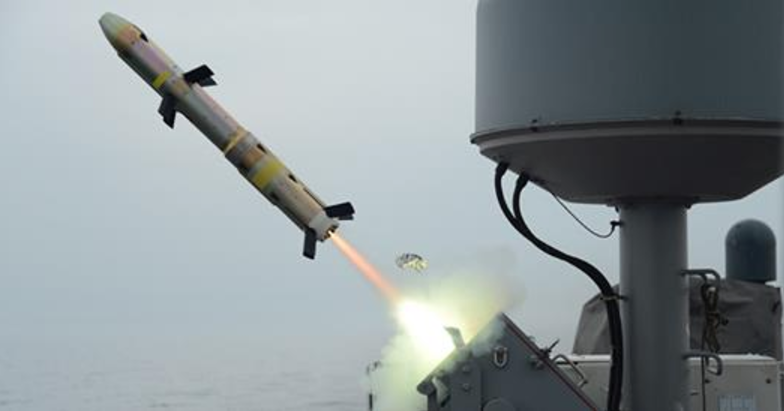
\includegraphics[width=5cm,frame]{griffinMissile}\newline
	\null\hfil\hfil\makebox[5cm]{Early Warning Radar}
	\hfil\hfil\makebox[5cm]{Raytheon AGM-176 Griffin}
	
	

	
	\subsection{Industry needs Robustness and Efficiency}
	For people in industry working on systems that can be modeled with Partial Differential Equations, there are a few key features for a solver that will make it more likely to be adopted:
	
	\begin{itemize}
		\item Solver must be fast
		\item Solver must be accurate
		\item Solver must be robust 
	\end{itemize}
	
	Those demands are lofty. Fortunately, Integral Equation based solvers make hitting all those targets feasible. Using Integral Equation based solvers, we can get great convergence rates, excellent conditioning properties, and the ability to accelerate computations using the Fast Multipole Method (FMM) and other hierarchical algorithms.
	

	% Dive into Maxwell Equation Formulation - MFIE
	
	\section{Electromagnetic Scattering on Perfect Conductors}
	\subsection{Fundamental Formulation}
	Many problems can be approximated as electromagnetic scattering with perfect conductors, so modeling these problems is our goal. Discussion on the modeling in the slides to come is based on \cite{dpie}.
	
	\vspace{0.1in}
	\begin{center}
		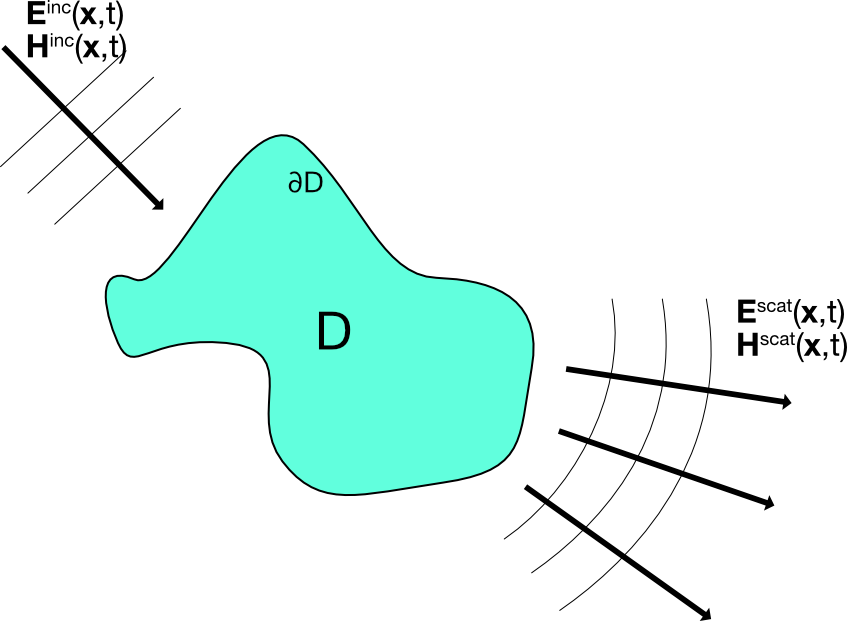
\includegraphics[width=7cm]{scatter_problem_pic}
	\end{center}
	
	For a fixed frequency $\omega$, the electric and magnetic fields, $\mathcal{E}$ and $\mathcal{H}$, take the form:
	
	\begin{align*}
	\mathcal{E}(\bvec{x},t) &= \mathcal{R}\lbrace \bvec{E}(\bvec{x}) e^{- i \omega t}\rbrace \\
	\mathcal{H}(\bvec{x},t) &= \mathcal{R}\lbrace \bvec{H}(\bvec{x}) e^{- i \omega t}\rbrace
	\end{align*}
	
	where $\mathcal{R}\lbrace z \rbrace$ returns the real part of $z$. We can then represent $\bvec{E}(\bvec{x})$ and $\bvec{H}(\bvec{x})$ as a sum of incident (known) and scattered (unknown) fields:
	
	\begin{align*}
	\bvec{E} &= \bvec{E}^{inc} + \bvec{E}^{scat} \\
	\bvec{H} &= \bvec{H}^{inc} + \bvec{H}^{scat}
	\end{align*}
	
	
	Given the above basic relationships, the system of equations to be solved take the form:
	
	\begin{itemize}
		\item Maxwell Equations
		\begin{align*}
		\nabla \times \bvec{E} = i \omega \mu \bvec{H}, \;\nabla \times \bvec{H} = - i \omega \epsilon \bvec{E}
		\end{align*}
		%
		\item Sommerfield-Silver-Müller Radiation Condition
		\begin{align*}
		\bvec{H}^{scat}(\bvec{x}) \times \frac{\bvec{x}}{|\bvec{x}|} - \sqrt{\frac{\mu}{\epsilon}} \bvec{E}^{scat}(\bvec{x}) = o(|\bvec{x}|^{-1}), \;\; |\bvec{x}| \rightarrow \infty
		\end{align*}
		%
		\item Perfect Conductor Boundary Conditions
		\begin{align*}
		\left(\bvec{n} \times \bvec{E}^{scat} \right)|_{\partial D} &= -\left( \bvec{n} \times \bvec{E}^{inc} \right)|_{\partial D} \\
		\left(\bvec{n} \cdot \bvec{H}^{scat} \right)|_{\partial D} &= -\left( \bvec{n} \cdot \bvec{H}^{inc} \right)|_{\partial D} 
		\end{align*}
	\end{itemize}
	
	These equations essentially give us what we need to make this problem well posed. For added convenience, however, some other useful relationships for modeling the problem are:
	
		\begin{align*}
		\left(\bvec{n} \cdot \bvec{E} \right)|_{\partial D} &= \frac{\rho}{\epsilon}|_{\partial D} \\
		\left(\bvec{n} \times \bvec{H} \right)|_{\partial D} &= \bvec{J}|_{\partial D} \\
		\nabla_s \cdot \bvec{J} &= i \omega \rho
		\end{align*}

	where $\bvec{J}$ and $\rho$ are the induced current density and charge on $\partial D$ and $\nabla_s \cdot \bvec{J}$ represents the surface divergence of the tangential current density. Using these extra relationships, one can formulate the solution to this system of equations in convenient ways.

	

	
	\subsection{Magnetic Field Integral Equation}
	\subsubsection{Formulation}
	The Magnetic Field Integral Equation (MFIE) can be used to model electromagnetic scattering for perfect conductors. The formulation begins by defining $\bvec{E}^{scat}$ and $\bvec{H}^{scat}$ using the Lorenz gauge vector and scalar potentials, $\bvec{A}^{scat}$ and $\phi^{scat}$
	
	\begin{align*}
	\bvec{E}^{scat} &= i \omega \bvec{A}^{scat} - \nabla \phi^{scat} \\
	\bvec{H}^{scat} &= \frac{1}{\mu} \nabla \times \bvec{A}^{scat}
	\end{align*}
	
	with the Lorenz gauge relationship defined as
	
	\begin{align*}
	\nabla \cdot \bvec{A}^{scat} &= i \omega \mu \epsilon \phi^{scat}
	\end{align*}
	
	We then define the $\bvec{A}^{scat}$ and $\phi^{scat}$ based on the induced surface current $\bvec{J}$ and charge $\rho$ using Single Layer Potentials in the following manner:
	
	\begin{align*}
	\bvec{A}^{scat}[\bvec{J}](\bvec{x}) &= \mu S_k [\bvec{J}](\bvec{x}) & \equiv \mu \int_{\partial D} g_k(\bvec{x} - \bvec{y}) \bvec{J}(\bvec{y})dA_y \\
	\bvec{\phi}^{scat}[\rho](\bvec{x}) &=\frac{1}{\epsilon} S_k [\rho](\bvec{x}) & \equiv \frac{1}{\epsilon} \int_{\partial D} g_k(\bvec{x} - \bvec{y}) \rho(\bvec{y})dA_y
	\end{align*}
	
	with $k = \omega \sqrt{\epsilon \mu}$ and the kernel being defined as:
	
	\begin{align*}
	g_k(\bvec{x}) &= \frac{e^{i k |\bvec{x}|}}{4 \pi |\bvec{x}|}
	\end{align*}
	
	
	We are able to do this because $\bvec{\phi}^{scat}$ and $\bvec{A}^{scat}$ are solutions to the scalar and vector Helmholtz equation. Now using $\bvec{H}^{scat} = \frac{1}{\mu} \nabla \times \bvec{A}^{scat}$ and the boundary condition
	
	\begin{align*}
	\left.\left(\bvec{n} \times \bvec{H} \right)\right|_{\partial D} &= \left.\bvec{J}\right|_{\partial D}
	\end{align*}
	
	the Magnetic Field Integral Equation can be found to be the following:
	
	\begin{align*}
	\frac{1}{2} \bvec{J}(\bvec{x}) - K[\bvec{J}](\bvec{x}) &= \bvec{n}(\bvec{x}) \times H^{inc}(x), \;\; \bvec{x} \in \partial D \\
	K[\bvec{J}](\bvec{x}) &= \int_{\partial D} \bvec{n}(\bvec{x}) \times \nabla \times g_k(\bvec{x} - \bvec{y}) \bvec{J}(\bvec{y}) dA_y \\
	\end{align*}
	
	After obtaining $\bvec{J}$, one can obtain $\rho$ by the integral equation shown below
	
	\begin{align*}
	\frac{1}{2} \rho(\bvec{x}) + G[\rho](\bvec{x}) &= \epsilon \bvec{n}(\bvec{x}) \cdot \bvec{E}^{inc} +  i \omega \epsilon \mu S_k[\bvec{J}](x), \;\; \bvec{x} \in \partial D \\
	G[\rho](\bvec{x}) &= \bvec{n} \cdot \nabla \int_{\partial D} g_k(\bvec{x} - \bvec{y}) \rho(\bvec{y}) dA_y \\
	\end{align*}
	
	Alternatively, you can back out $\phi^{scat}$ using the Lorenz gauge relationship:
	
	\begin{align*}
	\phi^{scat} &= -\frac{i}{\omega \epsilon} \nabla \cdot S_k[\bvec{J}]
	\end{align*} 
	
	and then use $\phi^{scat}$ and the integral operator form of $\bvec{A}^{inc}$ to get the scattered electromagnetic field. Either way you go about it, obtaining $\bvec{E}^{scat}$ and $\bvec{H}^{scat}$ is straight forward once you have $\bvec{J}$ and even more trivial if you also solve for $\rho$.
	
	


	
	\subsubsection{Problems with MFIE}
	Now why not just use the MFIE for these problems all the time? Well for starters, the MFIE is impacted by spurious resonances that make it so certain frequencies $\omega$ cause problems with arriving at a solution. Additionally, the MFIE is ill conditioned as $\omega \rightarrow 0$. To back out $\bvec{E}^{scat}$ and $\bvec{H}^{scat}$, need to perform computations with $\omega^{-1}$ which leads to catastrophic cancellation. For example, $\rho$ can be computed via the continuity equation, shown below, which obviously has a $\omega$ in the denominator.
	
	\begin{align*}
	\rho &= \frac{\nabla_s \cdot \bvec{J}}{i \omega \epsilon}
	\end{align*}
	
	One other interesting dilemma is that for $\omega = 0$ in multiply-connected domains, MFIE has a nonzero nullspace dimensionality equivalent to the genus of $\partial D$. This problem stems from the topology of the domain and is a problem with a non-obvious way to handle these errors.
	
	
	
	% looking at the DPIE
	
	\subsection{The Decoupled Potential Integral Equation}
	\subsubsection{Formulation}
	The premise for this formulation is to impose boundary conditions on the potentials $\phi$ and $\bvec{A}$ instead of the fields $\bvec{E}$ and $\bvec{H}$, in hopes the resulting integral equation can be better conditioned, insensitive to the topology of the domain, and remain straight forward to solve. First, the boundary conditions that will be imposed on the vector and scalar potentials are the following:
	
	\begin{align*}
	\left. \left(\bvec{n} \times \bvec{A}^{scat}\right)\right|_{\partial D} &= - \left. \left(\bvec{n} \times \bvec{A}^{inc}\right)\right|_{\partial D} \\
	\left. \left(\bvec{n} \times \nabla \phi^{scat}\right)\right|_{\partial D} &= - \left. \left(\bvec{n} \times  \nabla \phi^{inc}\right)\right|_{\partial D} \\
	\end{align*}
	
	These boundary conditions for the potentials can be shown to satisfy the Maxwell equations, radiation condition, and perfect conductor boundary conditions.
	Next is important to note that the Lorenz gauge condition does not uniquely determine what form the potentials $\bvec{A}$ and $\bvec{\phi}$ take. Due to this, $\bvec{A}$ and $\bvec{\phi}$ can be chosen to cast the problem into a more ideal form. For an incoming plane wave with a polarization vector $\bvec{E}_p$ and propagation direction $\bvec{u}$, the incident fields can be written as
	
	\begin{align*}
	\bvec{E}^{inc} &= \bvec{E}_p e^{i k \bvec{u} \cdot \bvec{x}} \\
	\bvec{H}^{inc} &= \sqrt{\frac{\epsilon}{\mu}} \bvec{u} \times \bvec{E}_p e^{i k \bvec{u} \cdot \bvec{x}}
	\end{align*}
	
	The standard potentials are $\bvec{A}^{inc} = \frac{\bvec{E}^{inc}}{i \omega}$, $\phi^{inc} = 0$, but these can be modified to the stable form
	
	\begin{align*}
	\bvec{A}^{inc} &= - \bvec{u} \left( \bvec{x} \cdot \bvec{E}_p\right) \sqrt{\mu \epsilon} e^{i k \bvec{u} \cdot \bvec{x}} \\
	\phi^{inc} &= - \bvec{x} \cdot \bvec{E}_p e^{i k \bvec{u} \cdot \bvec{x} }
	\end{align*}
	
	To  handle uniqueness of the vector potential solution $\bvec{A}^{scat}$ for all $k \geq 0$, the scalar Helmholtz is modified to
	
	\begin{align*}
	\Delta \phi^{scat} + k^2 \phi^{scat} &= 0 \\
	\phi^{scat}|_{\partial D_j} &= f + V_j \\
	\int_{\partial D_j} \left( \nabla \phi^{scat} \cdot \bvec{n}\right) ds &= Q_j
	\end{align*}
	
	where $f|_{\partial D_j} = - \phi^{inc}|_{\partial D_j}$ and $Q_j = - \int_{\partial D_j} \left( \nabla \phi^{inc} \cdot \bvec{n}\right) ds$. To handle uniqueness of the vector potential solution $\bvec{A}^{scat}$ for all $k \geq 0$, the vector Helmholtz is modified to
	
	\begin{align*}
	\Delta \bvec{A}^{scat} + k^2 \bvec{A}^{scat} &= 0 \\
	\left(\bvec{n} \times \bvec{A}^{scat}\right)|_{\partial D} &= \bvec{f} \\
	\bvec{n} \cdot \bvec{A}^{scat}|_{\partial D_j} &= h + v_j \\
	\int_{\partial D_j} \left( \bvec{n} \cdot \bvec{A}^{scat} \right) ds &= q_j
	\end{align*}
	
	where $\bvec{f}|_{\partial D_j} = - \bvec{n} \times \bvec{A}^{inc}|_{\partial D_j}$, $h = - \nabla \cdot \bvec{A}^{inc}|_{\partial D}$ and $q_j = - \int_{\partial D_j} \left( \bvec{n} \cdot \bvec{A}^{inc} \right) ds$. The modified formulations for the scalar and vector potentials are crucial to ensuring we have a unique solution and is especially useful with managing the topology issue that MFIE deals with. Now for convenience, note the following integral operator definitions:
	
	\begin{align*}
	S_k \sigma &= \int_{\partial D} g_k (\bvec{x} - \bvec{y}) \sigma(\bvec{y}) dA_y \\
	D_k \sigma &= \int_{\partial D} \frac{\partial g_k}{\partial n_y} (\bvec{x} - \bvec{y}) \sigma(\bvec{y}) dA_y \\
	S_k^{'} \sigma &= \int_{\partial D} \frac{\partial g_k}{\partial n_x}  (\bvec{x} - \bvec{y}) \sigma(\bvec{y}) dA_y \\
	D_k^{'} \sigma &= \frac{\partial }{\partial n_x}  \int_{\partial D} \frac{\partial g_k}{\partial n_y}  (\bvec{x} - \bvec{y}) \sigma(\bvec{y}) dA_y
	\end{align*}
	
	where $g_k(\bvec{x})$ is again defined as
	
	\begin{align*}
	g_k(\bvec{x}) &= \frac{e^{i k |\bvec{x}|}}{4 \pi |\bvec{x}|}
	\end{align*}
	
	After the modification to the scalar and vector Helmholtz, the scaled scalar potential DPIE (DPIEs) for is
	
	\begin{align*}
	\frac{\sigma}{2} + D_{k}\sigma - i k S_k \sigma - \sum_{j=1}^N V_j \chi_j &= f \\
	\int_{\partial D_j} \left( \frac{1}{k} D_{k}^{'} \sigma + i \frac{\sigma}{2} - i S_k^{'}\sigma \right) ds &= \frac{1}{k}Q_j
	\end{align*}
	
	with unknowns $\lbrace V_j\rbrace$, $\sigma$ for a representation of $\phi^{scat}(\bvec{x})$ as
	
	\begin{align*}
	\phi^{scat}(\bvec{x}) &= D_k [\sigma](\bvec{x}) - i k S_k [\sigma] (\bvec{x})
	\end{align*}
	
	Similarly, the scaled vector potential DPIE (DPIEv) is
	
	\begin{align*}
	\frac{1}{2}\begin{pmatrix}
	\bvec{a} \\
	\rho
	\end{pmatrix}
	+ 
	\bar{L} \begin{pmatrix}
	\bvec{a} \\
	\rho
	\end{pmatrix}
	+
	i \bar{R} \begin{pmatrix}
	\bvec{a} \\
	\rho
	\end{pmatrix}
	+ \begin{pmatrix}
	\bvec{0} \\
	\sum_{j=1}^N v_j \chi_j
	\end{pmatrix}
	&= \begin{pmatrix}
	\bvec{f} \\
	\frac{h}{k}
	\end{pmatrix} \\
	\int_{\partial D_j} \left(  \bvec{n} \cdot \nabla \times S_k\bvec{a} - k \bvec{n} \cdot S_k\left(\bvec{n} \rho \right) \right) ds + \;\;\;\;\;\;\;\;\;&\\
	i \int_{\partial D_j} \left(k \bvec{n} \cdot S_k\left(\bvec{n} \times \bvec{a}\right) - \frac{\rho}{2} + S_k^{'}\rho \right) ds &= q_j
	\end{align*}
	
	for $\bar{L}$ and $\bar{R}$ defined as 
	
	\begin{align*}
	\bar{L}\begin{pmatrix}
	\bvec{a} \\
	\rho
	\end{pmatrix}&= \begin{pmatrix}
	\bar{L}_{11} \bvec{a} + \bar{L}_{12} \rho \\
	\bar{L}_{21} \bvec{a} + \bar{L}_{22} \rho
	\end{pmatrix} \\
	%
	\bar{R} \begin{pmatrix}
	\bvec{a} \\
	\rho
	\end{pmatrix}  &= \begin{pmatrix}
	\bar{R}_{11} \bvec{a} + \bar{R}_{12} \rho \\
	\bar{R}_{21} \bvec{a} + \bar{R}_{22} \rho
	\end{pmatrix}
	\end{align*}
	
	where
	
	\begin{align*}
	\bar{L}_{11} \bvec{a} &= \bvec{n} \times S_k \bvec{a} & \bar{R}_{11} \bvec{a} &= k \bvec{n} \times S_k \bvec{n} \times \bvec{a}\\
	\bar{L}_{12} \rho &= - k \bvec{n} \times S_k\left(\bvec{n} \rho \right) & \bar{R}_{12} \rho &= \bvec{n} \times \nabla S_k\left( \rho \right)\\
	\bar{L}_{21} \bvec{a} &= 0 & \bar{R}_{21} \bvec{a} &= \nabla \cdot S_k \left(\bvec{n} \times \bvec{a}\right) \\
	\bar{L}_{22} \rho &= D_k \rho & \bar{R}_{22} \rho &= - k S_k \rho
	\end{align*}
	
	and we are tasked to find  unknowns $\lbrace v_j\rbrace$, $\bvec{a}$, $\rho$ for a representation of $\bvec{A}^{scat}(\bvec{x})$ as
	
	\begin{align*}
	\bvec{A}^{scat}(\bvec{x}) &= \nabla \times S_k[\bvec{a}](\bvec{x}) - k S_k[\bvec{n}\rho](\bvec{x}) \\
	&\;\;\;\; + i \left(k S_k[\bvec{n} \times \bvec{a}](\bvec{x}) + \nabla S_k[\rho](\bvec{x})\right)
	\end{align*}
	
	With the above system of integral equations for both the scalar and vector potentials, it is now feasible to use the DPIE formulation to handle arbitrary topologies for electromagnetic scattering problems under the perfect conductor assumption!

	% briefly discuss QBX
	
	\section{Quadrature by Expansion}
	The goal of QBX is to accurately handle evaluation of layer potential integrals on a boundary $\partial D$ where singularities can exist due to the integral operator kernel. 
	
	\hfil\hfil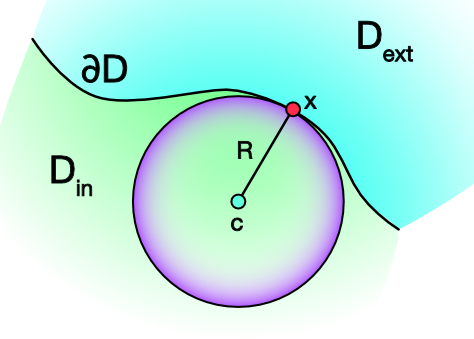
\includegraphics[width=5cm]{qbx_image}\hfil\hfil
	
	The idea is to perform an order $p$ expansion of some integral operator $K \sigma (\bvec{x})$ from some location $\bvec{c}$ and used that to evaluate $K \sigma(\bvec{x})$ at some boundary location $\bvec{x}$ where a singularity might exist. Given the field is smooth when restricted to the interior or exterior of the domain, this method is robust and accurate \cite{qbx}. 
	
	Using QBX, one can create robust and accurate discretizations of integral equations to solve for unknown densities at quadrature locations and can also robustly evaluate layer potentials for any representations one cares about. In the context of solving the DPIE system of integral equations, this method is worthwhile to use for both its robustness and accuracy properties. This is a big part of why this model is being implemented in the \textbf{pytential} Python package. \textbf{pytential} is founded upon using QBX for solving integral equations and has a collection of useful APIs for building new integral equation models that can benefit from QBX.
	
	\section{Software Implementation}
	The software for this DPIE model is being implemented for the Python package \textbf{pytential}. My forked version of this project can be found \href{https://github.com/choward1491/pytential}{here}, while the main package I am contributing to is found \href{https://github.com/inducer/pytential}{here}.
	
	Currently, a python class denoted as \textbf{DPIEOperator} is constructed that defined the system of integral equations for the scalar and vector potential unknown densities and unknown scalars tied to the topology. Additionally, the representations for $\phi^{scat}$, $\bvec{A}^{scat}$ as a function of their densities are implemented as part of this class. For convenience, this class can also be readily used to craft, using the density solutions of the DPIE system of equations, the resulting scattered electromagnetic fields $\bvec{E}^{scat}$ and $\bvec{H}^{scat}$.
	
	The above model still needs to be tested and so the associated test scripts are still being developed.
	
	\section{Numerical Results}
	As of writing this, no numerical results have yet been obtained. The current code is still in the process of being debugged and validated appropriately, but this report will be updated as progress is made. You can find the updated report at: 
	


	\newpage	
	\section{References}
	\begin{thebibliography}{9}
		\bibitem{dpie} 
		F. Vico, L. Greengard, M. Ferrando, and Z. Gimbutas. 
		\textit{The Decoupled Potential Integral Equation for Time-Harmonic Electromagnetic Scattering}. 
		2014. \\\texttt{https://arxiv.org/abs/1404.0749}
		
		\bibitem{qbx} 
		A. Klöckner, A. Barnett, L. Greengard, M. O'Neil.
		\textit{Quadrature by Expansion: A New Method for the Evaluation of Layer Potentials}.
		2013. \\\texttt{https://arxiv.org/abs/1207.4461}
		
	\end{thebibliography}
		
	



\end{document}